\chapter{Implementation}
\label{ch:implementation}

\section{The Projected Grid}
\label{sec_projected_grid}
The projected grid is based on a simple concept: in order to achieve an
uniform distribution of details on the image plane, a uniformly spaced grid is
created in post-perspective space and transformed back to world space.
Figure~\ref{fig:projectedgrid} illustrates the difference between a classic
world space approach and the projected grid.
\begin{figure}[h]
\centering
\subbottom[Classic]
{
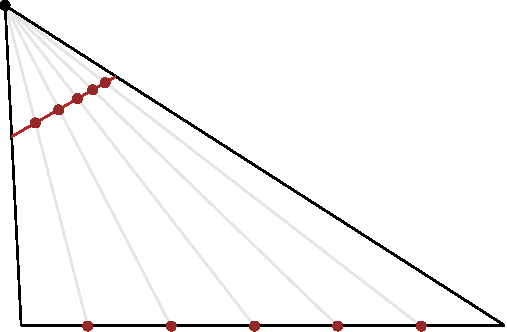
\includegraphics[scale=0.75]{figures/ProjectedGridVsWorldSpace.pdf}
\label{fig:subfigprojgrid1}
}
\subbottom[Projected Grid]
{
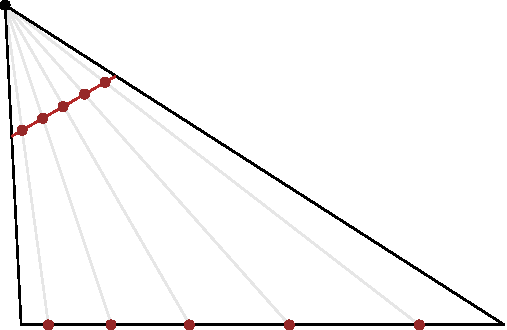
\includegraphics[scale=0.75]{figures/ProjectedGridUniform.pdf}
\label{fig:subfigprojgrid2}
}
\caption{The image on the left shows an uniform grid in worldspace,
its projection onto the image plane is not uniformly spaced though.
The image on the right on the other hand depicts an uniform grid on
the image plane and its associated non-uniform spaced worldspace
positions.}
\label{fig:projectedgrid}
\end{figure}

% The algorithm used for the projected grid can be broken down into the following
% steps:
% \begin{itemize}
%  \item create a uniformly spaced grid orthogonal to the viewer using normalised
% device coordinates
%  \item transform the grid to worldspace
%  \item project the grid onto the desired base plane
%  \item apply height displacement
%  \item run the grid through the rendering pipeline as usual
% \end{itemize}

\subsection{Coordinate Systems}
\label{sec:coordinate_systems}
Let $\mvec{x}$ be a vector representing the three dimensional carthesian
world space coordinate of a vertex, then
\begin{equation}
 \mvec{w} = \transpose{(\mvecx{x}, \mvecy{x}, \mvecz{x}, 1)}
\end{equation}
where $\mvec{w}$ is a homogeneous world space coordinate of $\mvec{x}$.
Let $\mmat{V}$ be the view matrix and $\mmat{P}$ the projection matrix, then
\begin{equation}
\label{eq:ws_to_cs}
 \mvec{c} = \mmat{P} \mmat{V} \mvec{w}
\end{equation}
where $\mvec{c}$ is the \textit{clip space} coordinate of $\mvec{w}$. For $\mvec{c}$ to
be inside the view frustum defined by $\mmat{P}$, $\mvec{c}$ is required to
meet the following condition
\begin{equation}
\label{eq:cs_bounds}
 \mvecx{c}, \mvecy{c}, \mvecz{c} \in \interval{-\mvecw{c}}{\mvecw{c}}
\end{equation}
where $\mvecw{c}$ is the homogeneous component of $\mvec{c}$. Next, clip space
vertex $\mvec{c}$ is transformed by the \textit{perspective division} as follows
\begin{equation}
\label{eq:cs_to_ndc}
 \mvec{n} = \frac{1}{\mvecw{c}}\transpose{(\mvecx{c}, \mvecy{c}, \mvecz{c})}
\end{equation}
where $\mvec{n}$ corresponds to the \textit{normalised device coordinate},
\textit{NDC} in short, of $\mvec{c}$.
%
%
\begin{figure}
\centering
\subbottom[View Frustum]
{
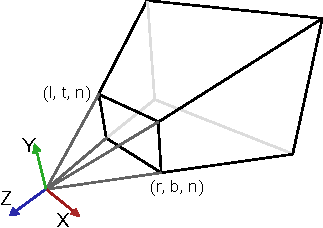
\includegraphics[width=0.4\textwidth]{figures/ProjectiveFrustum.pdf}
\label{fig:subfig_proj_frustum}
}
\subbottom[Canonical view volume]
{
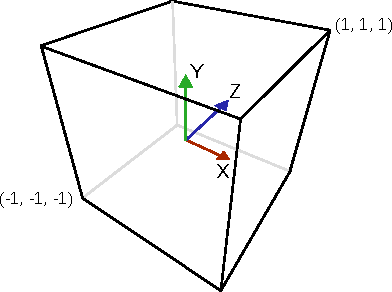
\includegraphics[width=0.4\textwidth]{figures/CanonicalCube.pdf}
\label{fig:subfig_canonical_view_volume}
}
\caption{Left: An example view frustum in view space. Right: The same view frustum
after applying projection and perspective division.}
\label{fig:proj_frustum_ndc}
\end{figure}
%
%
As one can see, equations~\ref{eq:cs_bounds}
and~\ref{eq:cs_to_ndc} imply
\begin{equation}
\label{eq:ndc_bounds}
 \mvecx{n}, \mvecy{n}, \mvecz{n} \in \interval{-1}{1}
\end{equation}
which defines the space NDC reside in, namely the \textit{canonical view volume},
see Figure~\ref{fig:proj_frustum_ndc}.\\


The projected grid, on the other hand, starts inside the canonical view volume
and needs to transform vertices back to world space. Let $\mvec{n}$ be the
normalised device coordinate of a vertex, then
\begin{equation}
\label{eq:ndc_to_cs}
 \mvec{c} = \transpose{(\mvecx{n}, \mvecy{n}, \mvecz{n}, 1)}
\end{equation}
where $\mvec{c}$ is a valid representation of $\mvec{n}$ in clip space. One may choose
a value for $\mvecw{c}$ different from $1$, making it necessary to scale $\mvecx{n}$,
$\mvecy{n}$ and $\mvecz{n}$ accordingly. Again, let $\mmat{V}$ be the view matrix and
$\mmat{P}$ the projection matrix, then
\begin{equation}
\label{eq:cs_to_wsh}
 \mvec{w} = \inverse{(\mmat{P} \mmat{V})} \mvec{c}
\end{equation}
where $\mvec{w}$ is a homogeneous world space coordinate of $\mvec{c}$. Conversion
to three dimensional carthesian world space is accomplished as follows
\begin{equation}
\label{eq:wsh_to_ws}
 \mvec{x} = \frac{1}{\mvecw{w}}\transpose{(\mvecx{w}, \mvecy{w}, \mvecz{w})}
\end{equation}

\subsection{Projection onto Plane}
As noted before, the vertices of the projected grid are represented as normalised
device coordinates. Assuming the plane the grid shall be projected on is specified
in world space coordinates, the following steps need to be computed for each vertex:
\begin{itemize}
 \item Transform vertex from canonical view volume to world space
 \item Setup vertex specific ray
 \item Intersect ray with target plane to compute actual position
\end{itemize}
Step one is already covered by Section~\ref{sec:coordinate_systems}. Step two
requires to setup a ray for each vertex, which implies both a position and a
direction. The position we already have, but to create a direction we need two
different positions. The solution is rather straightforward: let $\mvec{n}$ be
a \textit{two dimensional} vector representing the \textit{X} and \textit{Y}
components of a position in normalised device coordinates, then
\begin{align}
 \mvec{a} & = (\mvecx{n}, \mvecy{n}, -1, 1)\\
 \mvec{b} & = (\mvecx{n}, \mvecy{n}, +1, 1)
\end{align}
where $\mvec{a}$ corresponds to $\mvec{n}$ on the \textit{near plane} in clip space,
and $\mvec{b}$ to $\mvec{n}$ on the \textit{far plane} in clip space. Let $\mvec{d}$
and $\mvec{e}$ be the carthesian world space positions of $\mvec{a}$ and $\mvec{b}$
respectively, then
\begin{equation}
 \label{eq:proj_grid_ray}
 \mvec{p} = \mvec{d} + t(\mvec{e} - \mvec{d})
\end{equation}
where $\mvec{p}$ represents a ray starting at point $\mvec{d}$, pointing in direction
$(\mvec{e} - \mvec{d})$ with variable parameter $t$ controlling the actual position on
the ray.\\

Step three is about intersecting ray $\mvec{p}$ resulting from step two with the target plane.
We define the target plane using the \textit{Hesse normal form} as follows
\begin{equation}
\label{eq:proj_grid_plane}
 \mvec{p}\transpose{\mvec{n}} - d = 0
\end{equation}
where $\mvec{n}$ is the plane's normal vector with unit length and $d$ the plane's distance
from the origin. Next, we insert $\mvec{p}$ from equation~\ref{eq:proj_grid_ray}
into equation~\ref{eq:proj_grid_plane}, resulting in
%
\begin{gather}
\label{eq:plane_and_ray_intersection}
(\mvec{d} + t(\mvec{e} - \mvec{d})\transpose{\mvec{n}} - d = 0\\
\mvec{d}\transpose{\mvec{n}} + t(\mvec{e} - \mvec{d})\transpose{\mvec{n}} - d = 0\\
\intertext{solve for $t$}
t = \cfrac{d - \mvec{d}\transpose{\mvec{n}}}{(\mvec{e} - \mvec{d})\transpose{\mvec{n}}}
\end{gather}
%
where $t$ in combination with equation~\ref{eq:proj_grid_ray} gives the point of intersection
between the ray and the plane. In case $(\mvec{e} - \mvec{d})\transpose{\mvec{n}} = 0$,
there is no point of intersection because the ray is parallel to the plane.

\subsection{Projector}
\fxnote*{JÖSSAS}{Backfiring, etc}

\subsection{FFT}
Quadrant switching

Complex conjugate symmetry / Half-complex transform

Gradients

\begin{equation}
\eta(\mvec{x}, t) = 
\sum_{\mvec{k}}\frac{1}{\sqrt{2}}(\xi_r+\mathrm{i}\xi_i)
\sqrt{2\Theta(\mvec{k})\Delta k_x \Delta k_y} 
~\mathrm{e}^{-\mathrm{i}\omega(\mvec{k})t}
~\mathrm{e}^{\mathrm{i}\transpose{\mvec{k}}\mvec{x}}
\end{equation}

\begin{equation}
h_0(\mvec{k}) =
\frac{1}{2}
\frac{1}{\sqrt{2}}(\xi_r+\mathrm{i}\xi_i)
\sqrt{2\Theta(\mvec{k})\Delta k_x \Delta k_y}
\end{equation}

\begin{equation}
 h_0(\mvec{k}, t) =
 h_0(\mvec{k})\mathrm{e}^{-\mathrm{i}\omega(\mvec{k})t}
 + h_0^\ast(\mvec{-k})\mathrm{e}^{\mathrm{i}\omega(\mvec{k})t}
\end{equation}

Let $g(k)$ be the Fourier transform of $f(x)$, then we may write the
backward Fourier transform as follows:
\begin{equation}
 f(x) = \sum_{k}g(k)~\mathrm{e}^{\mathrm{i}kt}
\end{equation}
Note, that we omit the scaling factors involved in the Fourier transform
because in the context of this work they are not needed.
Given the backward Fourier transform, we may compute the derivative of $f(x)$
as follows:
\begin{equation}
  \diff{f(x)}{x} = \sum_{k}\mathrm{i}k~g(k)~\mathrm{e}^{\mathrm{i}kt}
\end{equation}
Let $n \in \mathbb{N}$, then the general rule for derivation is as follows:
\begin{equation}
  \diff[n]{f(x)}{x} = \sum_{k}(\mathrm{i}k)^n~g(k)~\mathrm{e}^{\mathrm{i}kt}
\end{equation}


\begin{align}
 f(\mvec{x}) &= \sum_{\mvec{k}}g(\mvec{k})~\mathrm{e}^{\mathrm{i}\transpose{\mvec{k}}\mvec{x}} \\
 \nabla f(\mvec{x}) &= \sum_{\mvec{k}}\mathrm{i}\mvec{k}~g(\mvec{k})~\mathrm{e}^{\mathrm{i}\transpose{\mvec{k}}\mvec{x}} \\
 \Rightarrow~&\diffp{f(\mvec{x})}{x} = \sum_{\mvec{k}}\mathrm{i}k_{x}~g(\mvec{k})~\mathrm{e}^{\mathrm{i}\transpose{\mvec{k}}\mvec{x}} \\
 &\diffp{f(\mvec{x})}{y} = \sum_{\mvec{k}}\mathrm{i}k_{y}~g(\mvec{k})~\mathrm{e}^{\mathrm{i}\transpose{\mvec{k}}\mvec{x}}
\end{align}

\begin{align}
\nabla\eta(\mvec{x},t) =
\sum_{\mvec{k}}&\mathrm{i}\mvec{k}~h_0(\mvec{k},t)
~\mathrm{e}^{\mathrm{i}\transpose{\mvec{k}}\mvec{x}} \\
\Rightarrow \frac{d\eta(\mvec{x},t)}{dx} &=
\sum_{\mvec{k}}\mathrm{i}k_x~h_0(\mvec{k},t)
~\mathrm{e}^{\mathrm{i}\transpose{\mvec{k}}\mvec{x}} \\
\frac{d\eta(\mvec{x},t)}{dy} &=
\sum_{\mvec{k}}\mathrm{i}k_y~h_0(\mvec{k},t)
~\mathrm{e}^{\mathrm{i}\transpose{\mvec{k}}\mvec{x}}
\end{align}

\begin{align}
\mvec{d}(\mvec{x},t) =
\sum_{\mvec{k}}&\mathrm{-i}\frac{\mvec{k}}{k}~h_0(\mvec{k},t)
~\mathrm{e}^{\mathrm{i}\transpose{\mvec{k}}\mvec{x}} \\
\Rightarrow d_x(\mvec{x},t) &=
\sum_{\mvec{k}}\mathrm{-i}\frac{k_x}{k}~h_0(\mvec{k},t)
~\mathrm{e}^{\mathrm{i}\transpose{\mvec{k}}\mvec{x}} \\
d_y(\mvec{x},t) &=
\sum_{\mvec{k}}\mathrm{-i}\frac{k_y}{k}~h_0(\mvec{k},t)
~\mathrm{e}^{\mathrm{i}\transpose{\mvec{k}}\mvec{x}}
\end{align}

\newcommand{\mcomplex}[2]{\ensuremath{{#1}{#2}\mathrm{i}}}

\begin{table}
\small
\setlength{\tabcolsep}{3.5pt} % default value: 6pt
\begin{tabular}{| S | S | S |}
\hline
0.30 & 0.72 & 1.00 \\
\hline
0.07 & 0.14 & 0.38 \\
\hline
0.16 & 0.12 & 0.33 \\
\hline
\end{tabular}
\quad
\sisetup{
round-mode      = places,
round-precision = 3,
}
\begin{tabular}{| S | S | S |}
\hline
\cellcolor{blue!25}        \num{-0.410 - 0.15588i} & \cellcolor{ProcessBlue!50}\num{1.42 - 0.01732i} & \cellcolor{Plum!50}        \num{-0.455 - 0.06062i}\\
\hline
\cellcolor{MidnightBlue!50}\num{-0.815 - 0.6322i}  & \cellcolor{red!50}\num{3.22 + 0.0i}     & \cellcolor{MidnightBlue!50}\num{-0.815 + 0.6322i}\\
\hline
\cellcolor{Plum!50}        \num{-0.455 + 0.06062i} & \cellcolor{ProcessBlue!50}\num{1.42 + 0.01732i} & \cellcolor{blue!25}        \num{-0.410 + 0.15588i}\\
\hline
\end{tabular}
\end{table}

\begin{table}
\small
\setlength{\tabcolsep}{3.5pt} % default value: 6pt
\begin{tabular}{| S | S | S | S |}
\hline
   0.85 &  0.57 &  0.98 &  0.18 \\
\hline
   0.85 &  0.68 &  0.36 &  0.79 \\
\hline
   0.27 &  0.48 &  0.79 &  0.17 \\
\hline
   0.86 &  0.35 &  0.66 &  0.78 \\
\hline
\end{tabular}
\quad
\sisetup{
round-mode      = places,
round-precision = 3,
}
\begin{tabular}{| S[table-number-alignment=right] | S[table-number-alignment=right] | S[table-number-alignment=right] | S[table-number-alignment=right] |}
\hline
\num{1.36000 + 0.00000i} & \cellcolor{ForestGreen!60}\num{-1.34000 + 1.24000i} & \num{-1.04000 + 0.00000i} & \cellcolor{ForestGreen!60}\num{-1.34000 - 1.24000i}\\
\hline
\cellcolor{Green!15}\num{0.67000 - 0.65000i} & \cellcolor{blue!25}\num{ 0.07000 + 0.37000i} & \cellcolor{ProcessBlue!50}\num{ 0.87000 + 0.03000i} & \cellcolor{Plum!50}\num{ 0.71000 + 0.21000i}\\
\hline
\num{1.62000 + 0.00000i} & \cellcolor{MidnightBlue!50}\num{ 0.04000 + 0.16000i} & \cellcolor{red!50}\num{ 9.62000 + 0.00000i} & \cellcolor{MidnightBlue!50}\num{ 0.04000 - 0.16000i}\\
\hline
\cellcolor{Green!15}\num{0.67000 + 0.65000i} & \cellcolor{Plum!50}\num{ 0.71000 - 0.21000i} & \cellcolor{ProcessBlue!50}\num{ 0.87000 - 0.03000i} & \cellcolor{blue!25}\num{ 0.07000 - 0.37000i}\\
\hline
\end{tabular}
\end{table}

Displacement

Displacement Derivatives
